\chapter[Sprint 1 : Socle applicatif et présélection]{Sprint 1 : Socle applicatif\\et présélection intelligente des candidats}
\begin{spacing}{1.2}
\minitoc%
\thispagestyle{MyStyle}
\end{spacing}
\clearpage

\providecommand{\screenshot}[2]{%
  \IfFileExists{../screenshoot/#1}{%
    \includegraphics[width=0.9\textwidth,height=12cm,keepaspectratio]{../screenshoot/#1}%
  }{%
    \fbox{\parbox[c][4.5cm][c]{0.9\textwidth}{\centering\itshape
      Capture d'écran à insérer~: #2\\[4pt]
      \normalfont\small(fichier attendu~: \texttt{screenshoot/#1})}}%
  }%
}

\section{Introduction}

Ce premier sprint pose les fondations de la plateforme NextHire. Il met en place l'environnement de développement, la structure du dépôt, le socle technique du back-end (API REST Node.js, authentification) et les briques de présélection des candidats~: analyse automatique des CV, recommandation d'offres et premiers écrans candidat et recruteur. À l'issue de ce sprint, un candidat peut s'inscrire, téléverser son CV et recevoir des offres recommandées, et un recruteur peut publier une offre.

\section{Objectifs du sprint}

L'objectif principal de ce sprint est défini comme suit~:

\begin{quote}
\itshape Établir les fondations techniques de la plateforme NextHire et son socle de présélection intelligente~: permettre à un candidat de s'inscrire, de téléverser son CV pour en extraire automatiquement un profil structuré et de recevoir des offres recommandées, et à un recruteur de publier une offre assortie d'un quiz de présélection.
\end{quote}

\subsection{Backlog du sprint}

Le tableau~\ref{tab:backlog-s1} présente le backlog de ce sprint~: les récits utilisateurs et tâches techniques sélectionnés depuis le \textit{product backlog} lors de la réunion de planification (\textit{sprint planning}). Comme pour le \textit{product backlog}, chaque élément est priorisé selon la méthode \textbf{MoSCoW} (\textbf{Must}, \textbf{Should}, \textbf{Could}) et estimé en \textit{story points} sur la suite de Fibonacci (1, 2, 3, 5, 8, 13), soit un engagement de 48~points pour ce sprint.

\begin{table}[H]
  \centering
  \footnotesize
  \renewcommand{\arraystretch}{1.3}
  \setlength{\tabcolsep}{5pt}
  \begin{tabularx}{\textwidth}{|>{\centering\arraybackslash}p{1.1cm}|>{\raggedright\arraybackslash}X|>{\centering\arraybackslash}p{1.7cm}|>{\centering\arraybackslash}p{0.9cm}|}
    \hline
    \rowcolor{blue!10}
    \textbf{ID} & \textbf{Récit utilisateur / tâche} & \textbf{Priorité} & \textbf{Est.} \\
    \hline
    T-01 & Initialiser le dépôt Git et la structure \textit{front-end} (React/Vite) et \textit{back-end} (Node.js/Express). & Must & 5 \\
    \hline
    S1 & En tant que candidat, je veux créer un compte et me connecter (JWT ou Google OAuth) afin d'accéder à la plateforme. & Must & 5 \\
    \hline
    S2 & En tant que candidat, je veux téléverser mon CV et obtenir automatiquement un profil structuré (extraction, OCR, analyse NLP). & Must & 8 \\
    \hline
    S3 & En tant que candidat, je veux consulter les offres d'emploi et soumettre une candidature. & Must & 3 \\
    \hline
    S4 & En tant que candidat, je veux recevoir des offres recommandées correspondant à mon profil. & Must & 5 \\
    \hline
    S5 & En tant que candidat, je veux relier mon compte LinkedIn afin d'enrichir mon profil. & Should & 3 \\
    \hline
    S6 & En tant que recruteur, je veux publier une offre d'emploi via l'assistant de création (\textit{Job Wizard}). & Must & 5 \\
    \hline
    S7 & En tant que candidat, je veux passer le quiz de présélection généré automatiquement pour ma candidature afin d'accéder à l'entretien. & Must & 5 \\
    \hline
    S8 & En tant que recruteur, je veux consulter le quiz de présélection de chaque candidature et le score obtenu par le candidat. & Must & 3 \\
    \hline
    S9 & En tant que candidat, je veux suivre le statut de ma candidature depuis mon tableau de bord afin de rester informé de son avancement. & Should & 3 \\
    \hline
    S10 & En tant que recruteur, je veux consulter la liste des candidatures et les profils détaillés afin d'étudier les candidats. & Must & 3 \\
    \hline
  \end{tabularx}
  \caption{Backlog du Sprint~1 : socle applicatif et présélection intelligente.}
  \label{tab:backlog-s1}
\end{table}

\section{Concept du socle de présélection}

Avant l'entretien proprement dit, NextHire filtre et qualifie les candidatures de façon \textit{intelligente}, sans se limiter à une recherche de mots-clés. Ce socle de présélection combine trois mécanismes complémentaires~: l'\textbf{analyse automatique du CV}, qui transforme un document hétérogène en profil structuré~; la \textbf{recommandation d'offres}, qui rapproche ce profil des postes ouverts par similarité sémantique et recouvrement de compétences~; et le \textbf{quiz de présélection}, qui vérifie objectivement les compétences déclarées avant l'accès à l'entretien.

L'ensemble s'appuie sur une base technique commune~: un \textit{front-end} React, un serveur Node.js jouant le rôle de point d'entrée unique, et une authentification centralisée qui oriente chaque utilisateur vers l'espace correspondant à son rôle (candidat, recruteur ou administrateur).

\section{Conception détaillée et architecture}

\subsection{Architecture du socle}

L'architecture micro-services et le pipeline de recommandation hybride ont été présentés en détail au chapitre~\ref{ch:sprint0} (Sprint~0). Ce sprint en concrétise le socle~: le serveur Node.js joue le rôle de point d'entrée unique (\textit{Backend For Frontend}), l'authentification est centralisée par jetons JWT, et la présélection des candidats repose sur deux micro-services Python indépendants, l'un dédié à l'analyse des CV, l'autre à la recommandation d'offres.

\subsection{Inscription, authentification et routage par rôle}

L'inscription crée un compte avec un rôle (candidat, recruteur ou administrateur)~; le mot de passe est haché par \texttt{bcrypt}. À la connexion, le serveur vérifie le mot de passe, signe un jeton JWT portant l'identité et le rôle, puis le client est routé vers l'espace correspondant (contrôle d'accès par rôle, RBAC). La figure~\ref{fig:seq-auth} illustre ce flux.

\begin{figure}[H]
  \centering
  \resizebox{0.85\textwidth}{!}{%
  \begin{tikzpicture}[
    font=\scriptsize, >={Stealth[length=2mm]},
    msg/.style={->, thin}, ret/.style={->, thin, dashed},
    lbl/.style={font=\tiny, fill=white, inner sep=1pt, midway, above},
    lifeline/.style={dashed, thin, gray!70},
    phdr/.style={draw, fill=blue!12, rounded corners=2pt, align=center,
                 font=\scriptsize\bfseries, minimum height=0.7cm, minimum width=2.8cm},
  ]
    \node[phdr] at ( 0,0) {Client\\(React)};
    \node[phdr] at ( 5,0) {Node BFF\\(:3001)};
    \node[phdr] at (10,0) {MongoDB};
    \foreach \x in {0,5,10}{ \draw[lifeline] (\x,-0.42) -- (\x,-8.0); }

    \draw[msg] ( 0,-0.85) -- node[lbl] {POST /api/auth/register \{email, rôle\}} (5,-0.85);
    \draw[->] (5,-1.35) -- ++(0.5,0) -- ++(0,-0.35) -- ++(-0.5,0);
    \node[font=\tiny, anchor=west] at (5.6,-1.52) {hacher le mot de passe (bcrypt)};
    \draw[msg] ( 5,-2.15) -- node[lbl] {insert User \{rôle\}} (10,-2.15);
    \draw[ret] (10,-2.75) -- node[lbl] {\{userId\}} (5,-2.75);
    \draw[ret] ( 5,-3.35) -- node[lbl] {201 Created} (0,-3.35);

    \draw[draw=gray!55, fill=gray!8, rounded corners=2pt, thin] (1.2,-3.75) rectangle (8.8,-4.2);
    \node[font=\tiny, anchor=west] at (1.3,-3.97) {Connexion ultérieure du candidat};

    \draw[msg] ( 0,-4.6) -- node[lbl] {POST /api/auth/login \{email, mot de passe\}} (5,-4.6);
    \draw[msg] ( 5,-5.2) -- node[lbl] {findOne(email)} (10,-5.2);
    \draw[ret] (10,-5.8) -- node[lbl] {\{user, hash\}} (5,-5.8);
    \draw[->] (5,-6.3) -- ++(0.5,0) -- ++(0,-0.35) -- ++(-0.5,0);
    \node[font=\tiny, anchor=west] at (5.6,-6.47) {vérifier bcrypt + signer le JWT \{id, rôle\}};
    \draw[ret] ( 5,-7.1) -- node[lbl] {200 OK \{token\}} (0,-7.1);
    \draw[->] (0,-7.6) -- ++(-0.5,0) -- ++(0,-0.0) ;
    \node[font=\tiny, anchor=west, text width=4.2cm] at (0.2,-7.75) {routage RBAC $\rightarrow$ espace candidat / recruteur / admin};
  \end{tikzpicture}}
  \caption{Diagramme de séquence : inscription, authentification et routage par rôle.}
  \label{fig:seq-auth}
\end{figure}

\subsection{Téléversement du CV, analyse et recommandation}

Le candidat téléverse son CV~; le serveur le confie à un micro-service d'analyse qui en extrait un profil structuré, puis sollicite le micro-service de recommandation pour proposer les offres les plus adaptées. La figure~\ref{fig:seq-cv-reco} détaille ce flux.

\begin{figure}[H]
  \centering
  \resizebox{\textwidth}{!}{%
  \begin{tikzpicture}[
    font=\scriptsize, >={Stealth[length=2mm]},
    msg/.style={->, thin}, ret/.style={->, thin, dashed},
    lbl/.style={font=\tiny, fill=white, inner sep=1pt, midway, above},
    lifeline/.style={dashed, thin, gray!70},
    phdr/.style={draw, fill=blue!12, rounded corners=2pt, align=center,
                 font=\scriptsize\bfseries, minimum height=0.7cm, minimum width=2.5cm},
  ]
    \node[phdr] at ( 0,0) {Candidat\\(React)};
    \node[phdr] at ( 4.5,0) {Node BFF\\(:3001)};
    \node[phdr] at ( 9,0) {Parseur CV\\(:5002)};
    \node[phdr] at (14,0) {Recommandation\\(:5001)};
    \node[phdr] at (18.5,0) {MongoDB};
    \foreach \x in {0,4.5,9,14,18.5}{ \draw[lifeline] (\x,-0.42) -- (\x,-8.6); }

    \draw[msg] ( 0,-0.85) -- node[lbl] {POST /api/users/cv (multipart)} (4.5,-0.85);
    \draw[->] (4.5,-1.35) -- ++(0.5,0) -- ++(0,-0.35) -- ++(-0.5,0);
    \node[font=\tiny, anchor=west] at (5.1,-1.52) {stocker le fichier (Multer)};
    \draw[msg] ( 4.5,-2.15) -- node[lbl] {POST /upload \{fichier\}} (9,-2.15);
    \draw[->] (9,-2.65) -- ++(0.5,0) -- ++(0,-0.35) -- ++(-0.5,0);
    \node[font=\tiny, anchor=west] at (9.6,-2.82) {extraction (pdfplumber / OCR) + NER};
    \draw[ret] ( 9,-3.45) -- node[lbl] {\{profil structuré\}} (4.5,-3.45);
    \draw[msg] ( 4.5,-4.05) -- node[lbl] {update User.profile} (18.5,-4.05);
    \draw[ret] ( 4.5,-4.65) -- node[lbl] {200 OK \{profil\}} (0,-4.65);

    \draw[draw=gray!55, fill=gray!8, rounded corners=2pt, thin] (1.5,-5.05) rectangle (12.5,-5.5);
    \node[font=\tiny, anchor=west] at (1.6,-5.27) {Recommandation d'offres pour le candidat};

    \draw[msg] ( 0,-5.9) -- node[lbl] {GET /recommendation/for-user} (4.5,-5.9);
    \draw[msg] ( 4.5,-6.5) -- node[lbl] {POST /recommend \{profil\}} (14,-6.5);
    \draw[->] (14,-7.0) -- ++(0.5,0) -- ++(0,-0.35) -- ++(-0.5,0);
    \node[font=\tiny, anchor=west] at (14.6,-7.17) {score hybride (FAISS + compétences)};
    \draw[ret] (14,-7.8) -- node[lbl] {\{offres classées\}} (4.5,-7.8);
    \draw[ret] ( 4.5,-8.4) -- node[lbl] {\{offres recommandées\}} (0,-8.4);
  \end{tikzpicture}}
  \caption{Diagramme de séquence : téléversement du CV, analyse et recommandation d'offres.}
  \label{fig:seq-cv-reco}
\end{figure}

\section{Réalisation et interfaces utilisateur}

\subsection{API REST du back-end}

Le backend Node.js (Express) expose une API REST organisée selon une convention de nommage
orientée ressources. L'ensemble des points de terminaison est regroupé sous le préfixe
\texttt{/api} et retourne des réponses JSON. Le serveur joue le rôle de point d'entrée unique
(\textit{Backend For Frontend}) : il monte une quinzaine de routeurs Express thématiques,
chacun responsable d'un domaine fonctionnel. Le tableau~\ref{tab:api-groups} récapitule les
principaux groupes de points de terminaison.

\begin{table}[H]
  \centering
  \footnotesize
  \renewcommand{\arraystretch}{1.3}
  \setlength{\tabcolsep}{5pt}
  \begin{tabularx}{\textwidth}{|>{\raggedright\arraybackslash}p{3.6cm}|>{\raggedright\arraybackslash}p{3.4cm}|>{\raggedright\arraybackslash}X|}
    \hline
    \rowcolor{blue!10}
    \textbf{Préfixe} & \textbf{Routeur} & \textbf{Rôle} \\
    \hline
    \texttt{/api/auth}, \texttt{/api/users} & \texttt{userRoute} & Connexion, inscription, OAuth Google, profils candidat et recruteur, enrôlement facial \\
    \hline
    \texttt{/api/jobs} & \texttt{jobRoute} & Gestion des offres d'emploi \\
    \hline
    \texttt{/api/wizard/jobs} & \texttt{jobWizardRoute} & Assistant de création d'offre (Job Wizard) \\
    \hline
    \texttt{/api/interviews} & \texttt{interviewRoute} & Cycle de vie de l'entretien, événements d'intégrité, rapports \\
    \hline
    \texttt{/api/call-rooms} & \texttt{callRoom} + \texttt{mediaRoute} & Sessions d'entretien IA, surveillance vision, enregistrements \\
    \hline
    \texttt{/api/job-rooms} & \texttt{jobInterviewRoom} & Salles d'entretien partageables, comparaison des candidats \\
    \hline
    \texttt{/quiz} & \texttt{quizRoute} & Quiz de présélection et modèles de quiz \\
    \hline
    \texttt{/api/messages} & \texttt{messages} & Messagerie temps réel recruteur / candidat \\
    \hline
    \texttt{/api/recommendations} & \texttt{recommendationRoute} & Recommandation d'offres basée sur le profil \\
    \hline
    \texttt{/api/recruiter/calendar}, \texttt{/api/internal/scheduling} & \texttt{recruiterCalendar}, \texttt{schedulingInternal} & Planification d'entretiens et intégration Google Calendar \\
    \hline
    \texttt{/api/linkedin} & \texttt{linkedinRoute} & Liaison et enrichissement du profil LinkedIn \\
    \hline
  \end{tabularx}
  \caption{Principaux groupes de points de terminaison REST du backend NextHire.}
  \label{tab:api-groups}
\end{table}

La validation des données entrantes est réalisée directement dans les gestionnaires de routes
et au niveau des schémas Mongoose, qui appliquent les contraintes de type, les champs requis,
les valeurs énumérées et l'unicité (par exemple l'adresse courriel). Plusieurs limiteurs de
débit (\texttt{express-rate-limit}), adossés en option à Redis, protègent les points de
terminaison sensibles tels que la génération de quiz par IA et la soumission des réponses.

\subsection{Authentification et autorisation}

L'authentification repose sur les jetons web JSON (JWT). Le déroulement est le suivant :

\begin{enumerate}
  \item Le client envoie une requête \texttt{POST /api/auth/login} avec son adresse courriel
        et son mot de passe.
  \item Le backend recherche l'utilisateur, vérifie le mot de passe haché avec
        \texttt{bcrypt}, puis génère un JWT signé contenant l'identifiant, l'adresse courriel
        et le rôle de l'utilisateur (\texttt{jwt.sign(\allowbreak\{id, email, role\}\allowbreak)}).
  \item Le client transmet ce JWT en tant que jeton \textit{Bearer} dans l'en-tête
        \texttt{Authorization} de toutes les requêtes suivantes.
  \item Le middleware \texttt{verifyToken} valide la signature et la date d'expiration du
        jeton avant de transmettre la requête ; toute requête non authentifiée reçoit une
        réponse \texttt{401}, de sorte que les gestionnaires métier ne traitent jamais de
        trafic anonyme.
  \item Le contrôle d'accès basé sur les rôles est assuré par le middleware
        \texttt{requireEnterprise} : les points de terminaison réservés au recruteur rejettent
        les requêtes au rôle candidat, avec un repli sur une vérification en base pour les
        jetons antérieurs ne portant pas encore le champ \texttt{role}.
\end{enumerate}

L'authentification via Google OAuth~2.0 est proposée comme méthode de connexion alternative.
Elle s'appuie sur la stratégie \texttt{passport-google-oauth20} : après autorisation de
l'utilisateur, le profil Google est récupéré via le \textit{callback}
\texttt{/auth/google/callback}, l'utilisateur est créé ou retrouvé en base, et un JWT
natif de la plateforme lui est délivré. Les jetons d'accès et de rafraîchissement Google sont
conservés pour permettre l'intégration ultérieure avec Google Calendar.

\subsection{Module d'extraction et d'analyse de CV}

Lorsqu'un candidat téléverse son CV, le fichier binaire (PDF ou image) est reçu par le
middleware \texttt{Multer} et stocké sur le système de fichiers local du serveur. L'analyse
est ensuite déléguée à un micro-service Python (Flask, port~5002) dédié, qui transforme un
document non structuré en un profil candidat exploitable par la plateforme.

\subsubsection{Extraction du texte (pipeline à deux niveaux)}

L'extraction du texte suit une stratégie en deux niveaux, choisie selon la nature du document~:

\begin{itemize}
  \item \textbf{Extraction native (PDF textuels).} La bibliothèque \texttt{pdfplumber} extrait
        le texte directement du PDF. Une reconstruction \textit{column-aware} a été développée
        pour traiter les CV sur deux colonnes~: un histogramme des positions horizontales des
        mots détecte l'espace inter-colonnes, puis le texte est recomposé colonne de gauche puis
        colonne de droite, afin d'éviter le mélange de lignes que produit l'ordre de lecture par
        défaut.
  \item \textbf{Reconnaissance optique (OCR) en repli.} Lorsque le texte natif est insuffisant
        (moins de 120~caractères ou de 20~mots) ou que le document est une image, le service
        rasterise chaque page avec \texttt{PyMuPDF} (facteur~2$\times$), puis applique
        \textbf{PaddleOCR} (modèle anglais, correction de l'orientation des lignes de texte)
        pour reconstruire le contenu. Le texte retenu est celui qui maximise la quantité
        d'information extraite.
\end{itemize}

Le texte obtenu est normalisé (suppression du bruit typographique, des artefacts
\texttt{(cid:n)} et des séparateurs) avant la phase d'analyse.

\subsubsection{Analyse et structuration du profil}

Le texte nettoyé est ensuite analysé par un pipeline de traitement du langage naturel combinant
la bibliothèque \texttt{spaCy} (modèle \texttt{en\_core\_web\_sm}) et un ensemble de règles et
d'expressions régulières bilingues (français/anglais). Ce pipeline extrait les champs
structurés du profil~: \texttt{name}, \texttt{email}, \texttt{phone}, \texttt{skills},
\texttt{languages}, \texttt{experience} (titre, entreprise, durée, description) et
\texttt{education}. Les compétences sont reconnues à partir d'un dictionnaire de référence
(\texttt{skills\_\allowbreak list.txt}), puis normalisées (par exemple \texttt{nodejs}~$\rightarrow$~%
\texttt{Node.js}) et filtrées par un validateur qui écarte les faux positifs (mots génériques,
fragments de phrases, encodages corrompus). Un \textbf{détecteur de domaine} classe enfin le
profil parmi dix familles métier (IA / \textit{Machine Learning}, \textit{data science},
développement logiciel, \textit{DevOps} / \textit{Cloud}, cybersécurité, finance, marketing,
ressources humaines, \textit{design} UX/UI et gestion de projet) par pondération des mots-clés rencontrés.

Pour écarter les documents qui ne sont pas des CV, un \textbf{classifieur binaire} valide le
résultat~: un modèle TF-IDF (n-grammes de 1 à 2) couplé à une régression logistique, entraîné
sur un jeu d'exemples étiquetés (CV contre factures, menus, relevés bancaires, etc.), produit
une probabilité d'appartenance à la classe «~CV~». Cette probabilité est combinée à des
heuristiques (présence de coordonnées, densité de mots-clés, présence de sections structurées)
pour accepter ou rejeter le document. Le profil validé est persisté dans le sous-document
\texttt{profile} de l'entité \texttt{User}, où il sert de contexte à l'agent d'entretien et au
moteur de recommandation décrit ci-après.

\subsection{Module de recommandation et de \textit{matching} d'offres}

Le \textit{matching} entre candidats et offres est assuré par un second micro-service Python
(Flask, port~5001) qui implémente une approche hybride combinant similarité sémantique et
recouvrement explicite des compétences.

\subsubsection{Représentation sémantique et indexation}

Chaque offre ouverte est convertie en un texte agrégé (titre, description, compétences,
langues) puis encodée en un vecteur dense de 384~dimensions par le modèle
\textbf{Sentence-Transformers} \texttt{all-MiniLM-L6-v2}. Si la bibliothèque n'est pas
disponible, le service bascule automatiquement sur un encodeur de repli
(\texttt{HashingVectorizer} de scikit-learn, 384~dimensions), ce qui garantit la continuité de
service. Les vecteurs sont normalisés et indexés dans un index \textbf{FAISS}
(\texttt{IndexFlatIP})~: le produit scalaire sur des vecteurs normalisés équivaut à une
similarité cosinus, ce qui permet une recherche des plus proches voisins efficace. L'index est
reconstruit périodiquement (toutes les heures, ou à la demande via un point d'accès dédié).

\subsubsection{Score hybride}

Le profil du candidat (résumé, compétences, langues, expériences) est encodé et normalisé de la
même manière, puis comparé à l'index FAISS pour obtenir un ensemble d'offres candidates avec
leur score sémantique. Le score final combine deux composantes~:
\[
  \text{score} = 0{,}25 \times \text{(similarité sémantique)} + 0{,}75 \times \text{(recouvrement pondéré des compétences)}.
\]
Le recouvrement des compétences est calculé après canonicalisation des intitulés (un
dictionnaire de synonymes ramène par exemple \texttt{js}, \texttt{reactjs} ou \texttt{node} à
leur forme canonique), puis pondéré~: chaque compétence porte un poids reflétant son importance
pour le poste (les technologies cœur comme React ou JavaScript pèsent davantage que des outils
secondaires). Une offre déjà candidatée par le candidat est exclue des résultats, et seules les
offres dont le score dépasse un seuil configurable (0{,}3 par défaut) sont retournées, classées
par pertinence décroissante. Chaque recommandation expose enfin le détail de son score
(part sémantique et part compétences), ce qui rend le \textit{matching} transparent pour le
candidat.

\subsection{Quiz de présélection et enrichissement LinkedIn}

En complément du \textit{matching}, le socle de présélection comprend un quiz technique de présélection. Dès qu'un candidat postule à une offre, un questionnaire personnalisé est généré automatiquement par l'IA (micro-service de génération de quiz) à partir des compétences attendues pour le poste et de celles du candidat, sans intervention du recruteur~; le candidat doit le réussir avant d'accéder à l'entretien, et les soumissions sont protégées par un limiteur de débit afin d'éviter les tentatives répétées. Par ailleurs, le candidat peut relier son compte LinkedIn à son profil~: un service d'enrichissement récupère ses données professionnelles publiques et complète automatiquement les compétences et expériences détectées dans le CV.

\subsection{Aperçu de l'interface utilisateur}

L'application cliente de NextHire est une application web monopage développée avec React~19
et empaquetée par Vite. Contrairement à une application de bureau, elle s'exécute
intégralement dans le navigateur et ne nécessite aucune installation. Le routage est assuré
par \texttt{react-router-dom}, qui distingue les espaces propres à chaque rôle : les écrans
candidat (profil, planification, salle d'entretien) et les écrans recruteur (espace
entreprise, salles d'entretien, comparaison des candidats), en plus d'un tableau de bord
d'administration.

La protection des routes et la gestion de session reposent sur un contexte React partagé,
\texttt{AuthContext}. À la connexion, le jeton JWT est conservé dans le \texttt{localStorage}
du navigateur, puis attaché à chaque appel au backend sous la forme d'un en-tête
\texttt{Authorization: Bearer <token>}. En cas de réponse signalant un jeton expiré ou
invalide, le contexte déconnecte l'utilisateur et le redirige vers la page de connexion. La
communication en temps réel (entretien, messagerie, alertes d'intégrité) s'appuie quant à
elle sur le client \texttt{socket.io-client}.

\subsection{Écrans candidat}

\subsubsection{Inscription et connexion}

L'accès à la plateforme commence par la page d'inscription et de connexion (routes \texttt{/register} et \texttt{/login}). Le candidat crée un compte avec son adresse courriel et un mot de passe, ou se connecte directement via \textbf{Google OAuth~2.0}. À l'authentification, le jeton JWT délivré par le serveur est conservé côté client et l'utilisateur est redirigé, selon son rôle, vers l'espace correspondant (figure~\ref{fig:login}).

\begin{figure}[H]
  \centering
  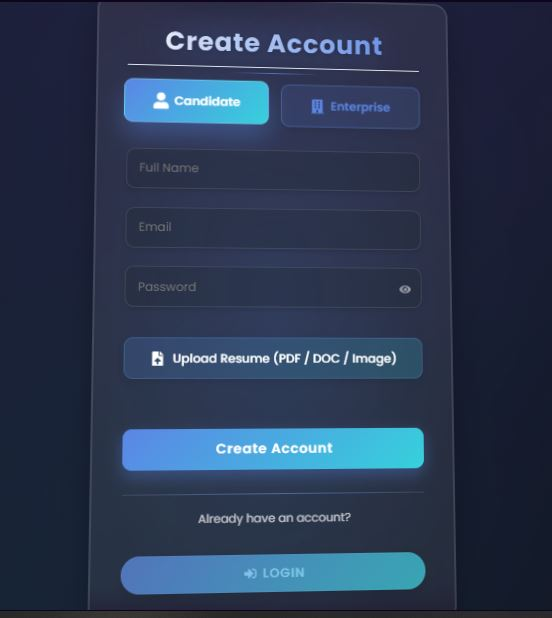
\includegraphics[width=0.48\textwidth,keepaspectratio]{../screenshoot/signup.JPG}\hfill
  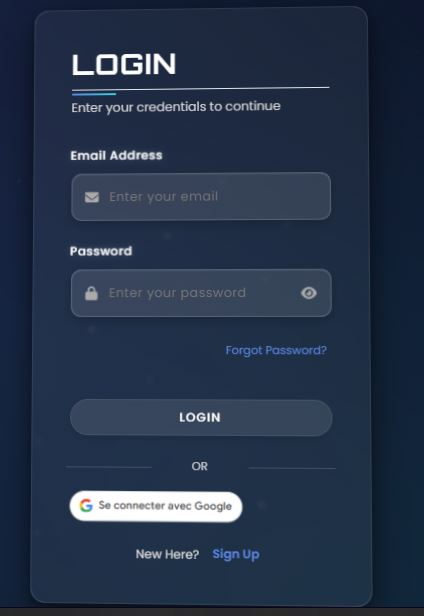
\includegraphics[width=0.48\textwidth,keepaspectratio]{../screenshoot/login.JPG}
  \caption{Écran d'inscription (à gauche) et de connexion (à droite) du candidat.}
  \label{fig:login}
\end{figure}

\subsubsection{Profil et tableau de bord candidat}

L'écran de profil candidat (route \texttt{/candidate/:id}) centralise les informations du
candidat : photo de profil vérifiée pour le contrôle d'identité, compétences, langues,
expériences et CV téléversé. Il présente également les candidatures soumises et les offres
recommandées par le moteur de recommandation. Un indicateur de complétude du profil incite
le candidat à compléter ses informations et à téléverser son CV, étape nécessaire avant de
postuler (figure~\ref{fig:candidate-profile}).

\begin{figure}[H]
  \centering
  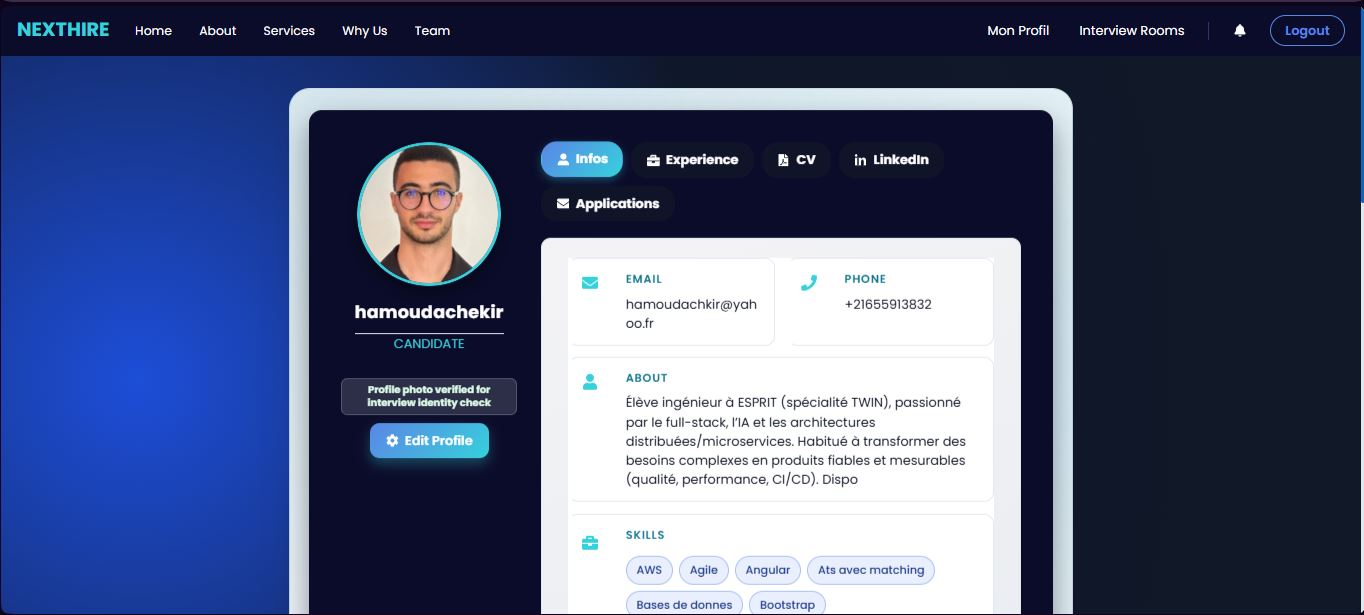
\includegraphics[width=0.48\textwidth,keepaspectratio]{images/profile1.JPG}\hfill
  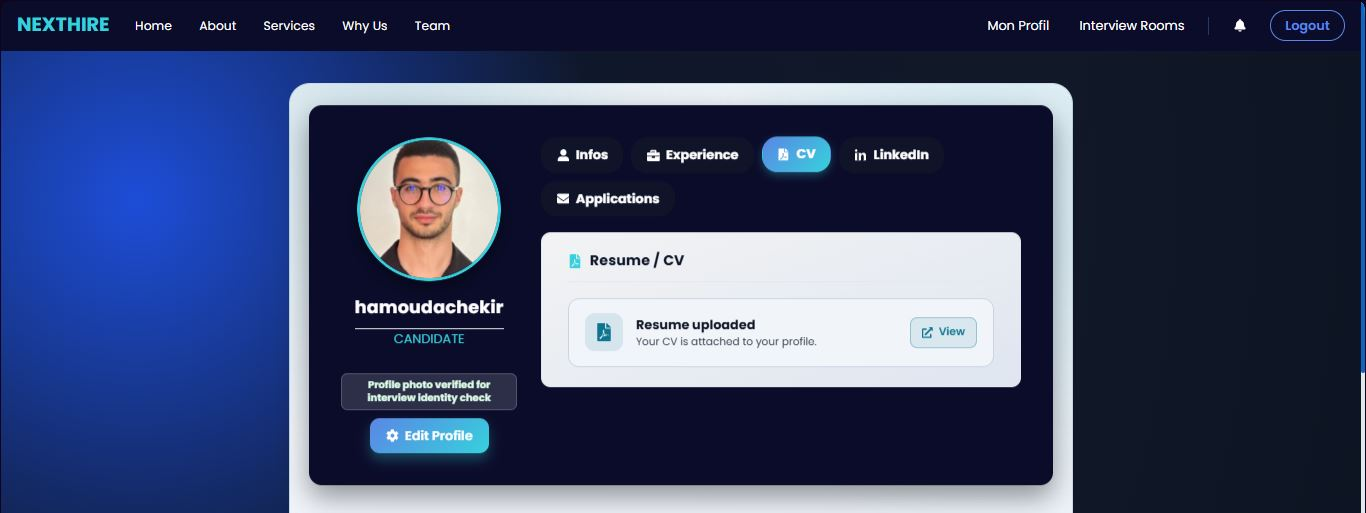
\includegraphics[width=0.48\textwidth,keepaspectratio]{images/profile2.JPG}\\[6pt]
  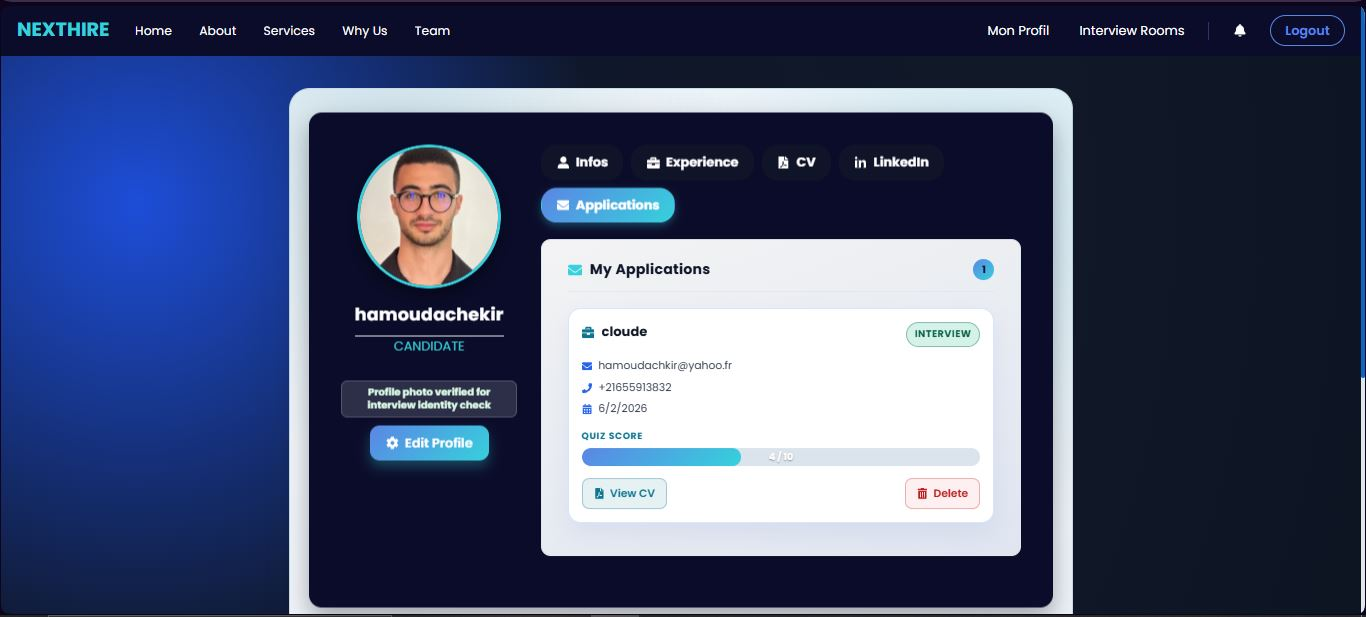
\includegraphics[width=0.75\textwidth,keepaspectratio]{images/profile3.JPG}
  \caption{Écran de profil et tableau de bord du candidat.}
  \label{fig:candidate-profile}
\end{figure}

\subsubsection{Téléversement du CV et profil structuré}

Depuis son profil, le candidat téléverse son CV (PDF ou image). Le fichier est transmis au micro-service d'analyse décrit précédemment, qui en extrait automatiquement un profil structuré : identité, compétences, langues, expériences et formation. Le candidat peut ensuite vérifier et compléter les informations détectées avant de postuler (figure~\ref{fig:cv-upload}).

\begin{figure}[H]
  \centering
  \screenshot{cv-upload.JPG}{Téléversement du CV et profil extrait automatiquement}
  \caption{Téléversement du CV et profil structuré extrait automatiquement.}
  \label{fig:cv-upload}
\end{figure}

\subsubsection{Liaison du compte LinkedIn}

En complément du CV, le candidat peut relier son compte LinkedIn à son profil. Un service d'enrichissement récupère ses données professionnelles publiques et complète automatiquement les compétences et expériences détectées, ce qui améliore la qualité de la présélection et des recommandations (figure~\ref{fig:linkedin}).

\begin{figure}[H]
  \centering
  \screenshot{linkedin-enrichment.JPG}{Liaison du compte LinkedIn et enrichissement du profil}
  \caption{Liaison du compte LinkedIn et enrichissement automatique du profil.}
  \label{fig:linkedin}
\end{figure}

\subsubsection{Page d'accueil et recommandation d'offres}

Dès sa connexion, le candidat arrive sur une page d'accueil qui met en avant une liste
d'offres recommandées personnalisées (figure~\ref{fig:candidate-home}). Le \textit{front-end}
React interroge la route \texttt{GET /recommendation/for-user}, qui relaie la requête au
micro-service de recommandation Python (port~5001) décrit au chapitre~\ref{ch:sprint0} (Sprint~0). Pour la page
d'accueil, le backend demande jusqu'à dix offres (\texttt{top\_k}~=~10) avec un seuil de
similarité abaissé à $0{,}2$ (au lieu de $0{,}3$ par défaut), afin d'élargir l'éventail
d'offres proposées au candidat.

Chaque offre est restituée avec son score de correspondance (\texttt{match\_score}) issu du
score hybride, et les informations de l'entreprise (nom, logo) sont jointes en une seule
requête à la base de données pour enrichir l'affichage. Les offres auxquelles le candidat a
déjà postulé sont automatiquement écartées par le service de recommandation. Le candidat peut
alors consulter le détail d'une offre et postuler directement depuis cette page. Pour préserver
la robustesse de l'interface, l'API se comporte de façon dégradée : si le service de
recommandation est momentanément indisponible, elle renvoie une liste vide plutôt qu'une
erreur, et la page d'accueil reste fonctionnelle.

\begin{figure}[H]
  \centering
  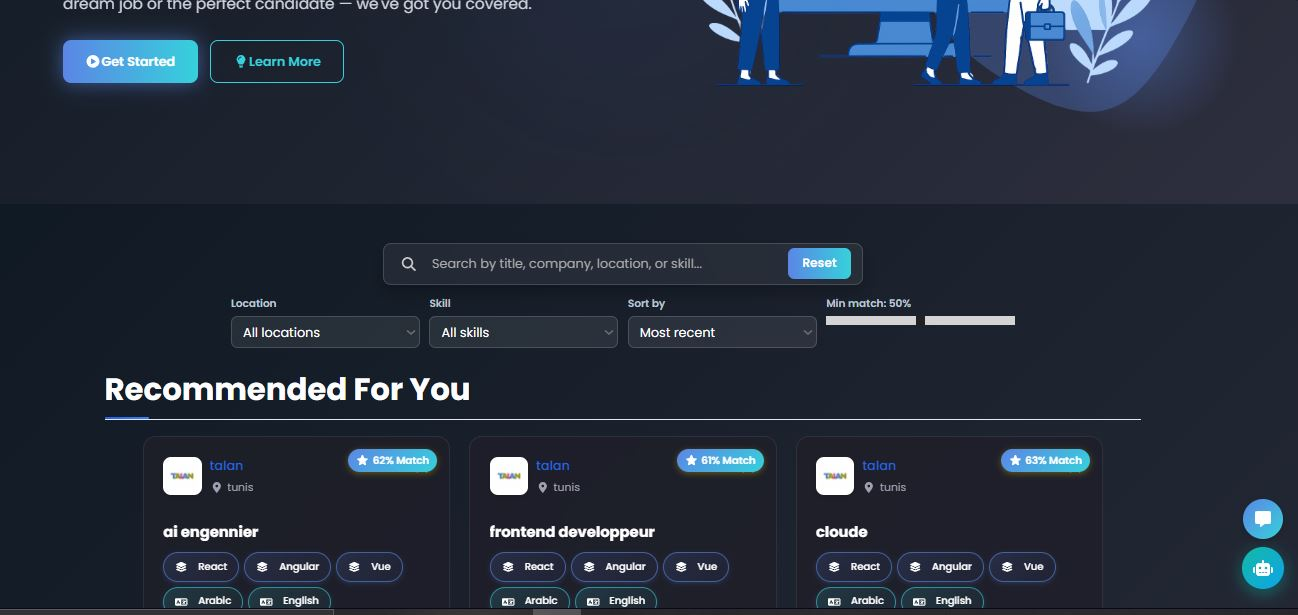
\includegraphics[width=0.9\textwidth,keepaspectratio]{images/home.JPG}
  \caption{Page d'accueil candidat avec les offres recommandées.}
  \label{fig:candidate-home}
\end{figure}

\subsubsection{Quiz de présélection}

Avant d'accéder à l'entretien, le candidat doit réussir le quiz de présélection généré pour sa candidature. Le questionnaire, personnalisé et généré automatiquement par l'IA dès la candidature à partir des compétences attendues pour le poste et de celles du candidat, présente une série de questions (QCM, vrai/faux, réponse courte, mini-exercice) à durée limitée~; le nombre de tentatives est plafonné par un limiteur de débit. Le score obtenu conditionne l'accès à l'étape suivante (figure~\ref{fig:quiz-candidat}).

\begin{figure}[H]
  \centering
  \screenshot{quiz-candidat.JPG}{Passage du quiz de présélection côté candidat}
  \caption{Passage du quiz de présélection par le candidat.}
  \label{fig:quiz-candidat}
\end{figure}

\subsection{Écrans recruteur}

\subsubsection{Tableau de bord recruteur}

L'espace recruteur (route \texttt{/entreprise/:id}, composant \texttt{EntrepriseProfile})
présente les offres d'emploi publiées par l'entreprise, le nombre de candidatures par offre
et la liste des candidats associés. Le recruteur peut y créer ou modifier une offre grâce à
l'assistant de création (\textit{Job Wizard}), suivre l'avancement des candidatures et
accéder au profil de chaque candidat (figure~\ref{fig:recruiter-dashboard}).

\begin{figure}[H]
  \centering
  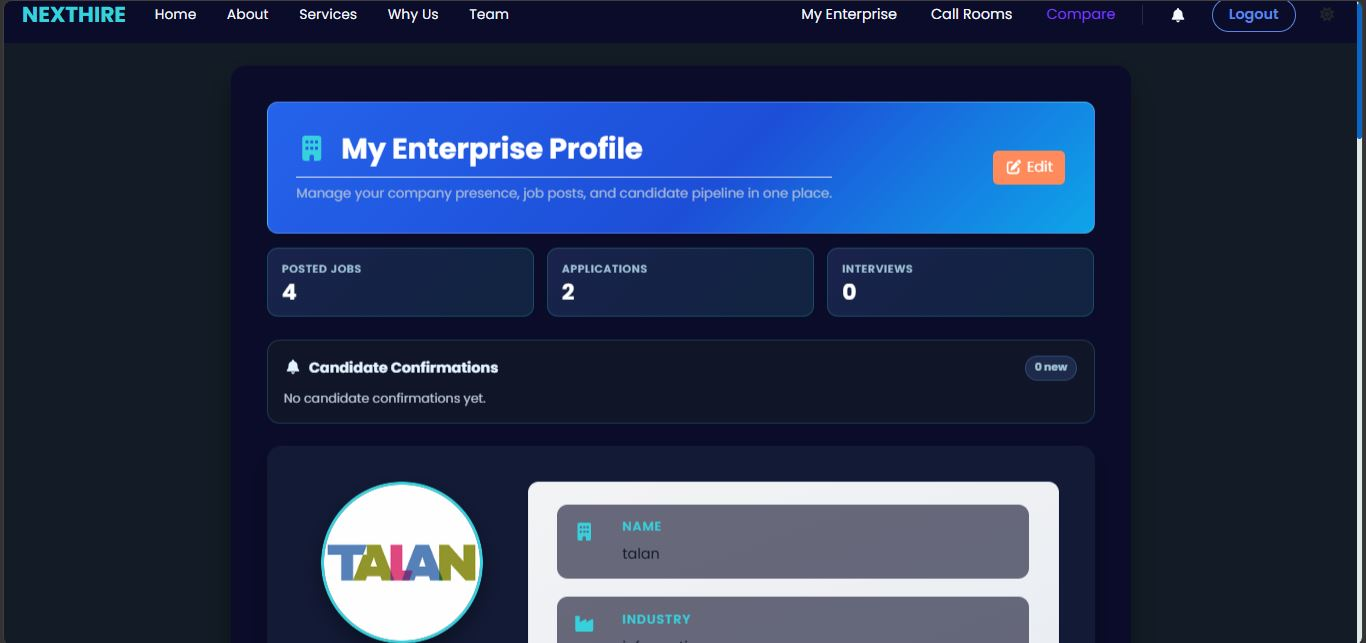
\includegraphics[width=0.9\textwidth,keepaspectratio]{../screenshoot/profilentre.JPG}\\[6pt]
  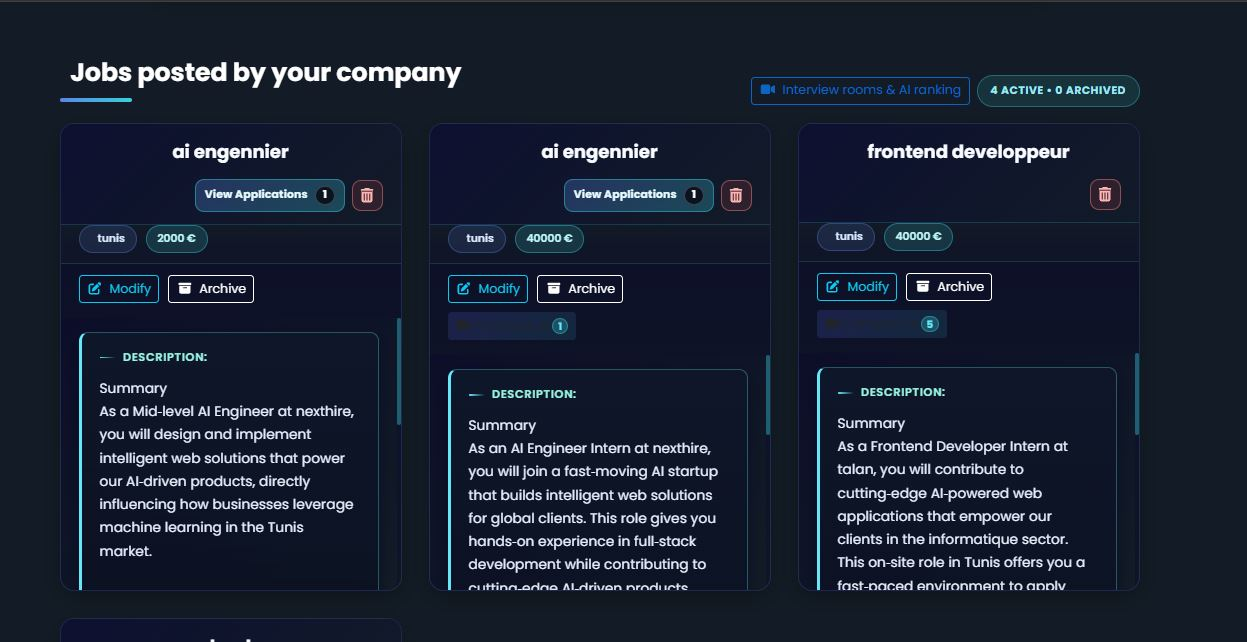
\includegraphics[width=0.9\textwidth,keepaspectratio]{../screenshoot/profjiob.JPG}
  \caption{Tableau de bord recruteur avec vue des offres et des candidatures.}
  \label{fig:recruiter-dashboard}
\end{figure}

\subsubsection{Création d'une offre avec le Job Wizard}

La création d'une offre s'effectue via l'assistant de création (\textit{Job Wizard}), un parcours guidé en plusieurs étapes assisté par l'IA. Le recruteur y renseigne le titre, la description, les compétences requises et le niveau de séniorité~; l'assistant propose des suggestions de contenu et configure les critères d'évaluation pondérés de l'entretien. Le quiz de présélection n'intervient pas à cette étape~: il sera généré automatiquement, par candidat, au moment où celui-ci postule à l'offre (figure~\ref{fig:job-wizard}).

\begin{figure}[H]
  \centering
  \screenshot{job-wizard.JPG}{Assistant de création d'offre (Job Wizard) assisté par IA}
  \caption{Création d'une offre d'emploi via l'assistant \textit{Job Wizard}.}
  \label{fig:job-wizard}
\end{figure}

\section{Tests}

À ce stade du projet, la validation s'est appuyée sur des tests manuels des points de terminaison REST réalisés avec Postman~: création de compte, connexion par JWT, téléversement et analyse de CV, génération des recommandations d'offres et publication d'une offre côté recruteur. Le parcours d'inscription et de complétion de profil a par ailleurs été vérifié de bout en bout dans le navigateur. Les suites de tests automatisées, mutualisées à l'échelle de la plateforme, sont présentées au chapitre~\ref{ch:sprint5} (Sprint~5).

\section{Conclusion}

Ce sprint a livré un socle fonctionnel~: inscription, authentification, analyse de CV, recommandation d'offres et quiz de présélection, ainsi que les premiers espaces candidat et recruteur. Conformément au cadre Scrum, cet incrément a été démontré à nos encadrantes lors de la revue de sprint~; la rétrospective a notamment mis en évidence la grande hétérogénéité des CV réels, ce qui a conduit à renforcer le pipeline d'extraction (reconstruction par colonnes, repli OCR) et à constituer des jeux d'essai plus variés pour les sprints suivants. Le sprint suivant s'appuie sur ces fondations pour introduire la planification des entretiens et la première version de la salle d'entretien en temps réel.
